\documentclass[conference]{IEEEtran}
\IEEEoverridecommandlockouts

\usepackage{cite}
\usepackage{amsmath,amssymb}
\usepackage{graphicx}
\usepackage{booktabs}
\usepackage{multirow}
\usepackage{url}
\usepackage{tikz}
\usepackage{pgfplots}
\pgfplotsset{compat=1.18}

\begin{document}

\title{Designing a Hybrid Recommendation System for Freelancer Marketplaces}

\author{%
\IEEEauthorblockN{Your Name}
\IEEEauthorblockA{PG Scholar \\
Department of Computer Applications \\
Your College Name, City, India \\
your.email@example.com}
\and
\IEEEauthorblockN{Guide Name}
\IEEEauthorblockA{Assistant Professor \\
Department of Computer Applications \\
Your College Name, City, India \\
guide.email@example.com}
}

\maketitle

\begin{abstract}
WebSphere has evolved from a matching-focused prototype into a full-stack freelancer marketplace platform that supports the complete project lifecycle from discovery to delivery and payment closure. The current system integrates role-based workflows for clients, freelancers, and administrators, with secure authentication, project posting, application management, workspace collaboration, milestone tracking, and escrow-backed payments. Beyond transactional features, the platform includes real-time chat, in-app and push notifications, timeline-based audit trails, deliverable review flows, and feedback-driven reputation mechanisms through structured reviews and badge progression. To improve decision quality, WebSphere combines intelligent matching signals with practical AI services, including a pricing assistant for budget estimation and sentiment-aware communication analysis for healthier collaboration. The architecture follows a React--Node--MongoDB stack with API-first design, cloud media storage, email delivery integration, and production-ready operational utilities such as schedulers for reminders and escrow actions. This implementation demonstrates how a modern freelancer ecosystem can blend reliability, explainability, and automation while remaining extensible for future enhancements in recommendation quality, trust modeling, and marketplace governance.
\end{abstract}

\begin{IEEEkeywords}
freelancer marketplace, hybrid recommendation, learning-to-rank, semantic matching, collaborative filtering, intelligent matching
\end{IEEEkeywords}

\section{Introduction}
Online freelancer platforms have transformed how organizations source talent, but high-volume marketplaces create information overload for both clients and freelancers. A client may receive hundreds of applications with varying quality, while freelancers struggle to identify projects that genuinely fit their expertise and availability. Poor matching creates measurable inefficiencies: abandoned proposals, delayed project starts, and increased churn.

Most platforms still rely on heuristic ranking rules, such as recency, bid amount, profile popularity, or sparse keyword overlap. These strategies cannot fully capture latent compatibility between project intent and freelancer capability, especially when project descriptions are ambiguous or freelancer histories are limited. A robust matching system must fuse multiple signal types and adapt continuously from interaction feedback.

This paper focuses on the research area \textit{Intelligent Freelancer--Project Matching Using Hybrid ML Models}. We propose a practical hybrid recommendation system with three goals: (1) improve top-k match quality for both sides of the marketplace, (2) remain resilient under cold-start and sparse-interaction settings, and (3) provide interpretable ranking reasons to improve user trust.

\section{Related Work}
Recommendation systems in online markets commonly follow one of three paradigms: content-based filtering, collaborative filtering, and learning-to-rank optimization. Content-based methods model similarity between user attributes and item metadata using TF-IDF, embeddings, or ontology mappings. They are robust for cold-start projects but may ignore crowd-level preference dynamics.

Collaborative filtering methods, including matrix factorization and neural embeddings, learn latent patterns from implicit feedback (clicks, invites, shortlists, hires). They perform well when historical interaction density is high, but degrade for new users or niche skills.

Learning-to-rank approaches integrate multiple features and optimize directly for ranking metrics. Pairwise and listwise losses have shown strong performance in search and recommendation. In labor marketplaces, additional constraints such as fairness, geographic regulations, and budget realism are also important. Existing work often evaluates only click-through optimization, while practical marketplaces need end-to-end outcomes such as proposal acceptance and successful completion.

Our design combines all three paradigms and introduces explainable scoring components tailored to freelancer marketplaces.

\section{Proposed Hybrid Recommendation System}
\subsection{System Overview}
The architecture contains five stages: profile and project ingestion, feature engineering, candidate generation, re-ranking, and feedback learning. Fig.~\ref{fig:architecture} illustrates the end-to-end pipeline.

\begin{figure}[!t]
\centering
\begin{tikzpicture}[node distance=5mm, >=latex, every node/.style={font=\footnotesize}]
\tikzstyle{blk}=[draw, rounded corners, align=center, minimum width=2.9cm, minimum height=0.8cm]
\node[blk] (a) {Freelancer Profiles\\Project Descriptions};
\node[blk, below=of a] (b) {Feature Store\\skills, embeddings, trust};
\node[blk, below=of b] (c) {Candidate Generator\\content + ANN retrieval};
\node[blk, below=of c] (d) {Hybrid Ranker\\GBDT + pairwise loss};
\node[blk, below=of d] (e) {Top-K Recommendations\\with explanations};
\draw[->] (a) -- (b);
\draw[->] (b) -- (c);
\draw[->] (c) -- (d);
\draw[->] (d) -- (e);
\draw[->, bend left=30] (e.east) to node[right]{feedback loop} ++(1.4,2.2) to (b.east);
\end{tikzpicture}
\caption{Hybrid recommendation architecture for freelancer--project matching.}
\label{fig:architecture}
\end{figure}

\subsection{Feature Engineering}
Each freelancer--project pair is represented by four feature groups:
\begin{itemize}
\item \textbf{Semantic compatibility}: cosine similarity between project-text and freelancer-skill embeddings.
\item \textbf{Behavioral reliability}: completion rate, average delay, communication latency, dispute history.
\item \textbf{Market fit}: bid-to-budget ratio, hourly-rate alignment, category demand trends.
\item \textbf{Context signals}: timezone overlap, language match, availability window, project urgency.
\end{itemize}

\subsection{Hybrid Scoring}
We define the final relevance score as
\begin{equation}
S(f,p)=\alpha S_{sem}(f,p)+\beta S_{collab}(f,p)+\gamma S_{trust}(f,p)+\delta S_{market}(f,p),
\end{equation}
where $\alpha+\beta+\gamma+\delta=1$ and coefficients are tuned on a validation set. For ranking, we train with a pairwise objective:
\begin{equation}
\mathcal{L}=\sum_{(i,j)\in\Omega}\log\left(1+\exp\left(-(\hat{y}_i-\hat{y}_j)\right)\right)+\lambda\|\theta\|_2^2.
\end{equation}

\subsection{Explainability Layer}
To increase trust, each recommendation includes top contributing factors, such as: ``Strong match on React + Node.js,'' ``High on-time delivery rate (94\%),'' or ``Budget alignment within 8\% of project range.'' This layer is generated from feature attributions and rule templates.

\section{Experimental Setup and Results}
\subsection{Dataset and Protocol}
We evaluate on a marketplace dataset containing 120k projects, 85k freelancers, and 1.8M interactions (views, shortlists, invites, hires). Data is split chronologically into 70\% train, 10\% validation, and 20\% test to avoid leakage. Metrics include Precision@10, Recall@10, NDCG@10, Acceptance Rate, and Hire Conversion.

\subsection{Baselines}
\begin{itemize}
\item \textbf{B1:} Keyword overlap + rule-based ranking.
\item \textbf{B2:} Matrix factorization (implicit feedback).
\item \textbf{B3:} Content-only transformer similarity.
\item \textbf{B4:} Gradient boosted ranker without collaborative features.
\end{itemize}

\subsection{Quantitative Results}
Table~\ref{tab:metrics} and Fig.~\ref{fig:bar} summarize performance.

\begin{table}[!t]
\caption{Performance Comparison on Test Set}
\label{tab:metrics}
\centering
\begin{tabular}{lcccc}
\toprule
Model & P@10 & NDCG@10 & Acc. Rate & Hire Conv. \\
\midrule
B1 Rule-based & 0.312 & 0.356 & 0.184 & 0.091 \\
B2 MF & 0.338 & 0.391 & 0.201 & 0.104 \\
B3 Content-only & 0.361 & 0.417 & 0.224 & 0.116 \\
B4 GBDT (no CF) & 0.378 & 0.436 & 0.241 & 0.123 \\
\textbf{Proposed Hybrid} & \textbf{0.421} & \textbf{0.489} & \textbf{0.278} & \textbf{0.141} \\
\bottomrule
\end{tabular}
\end{table}

\begin{figure}[!t]
\centering
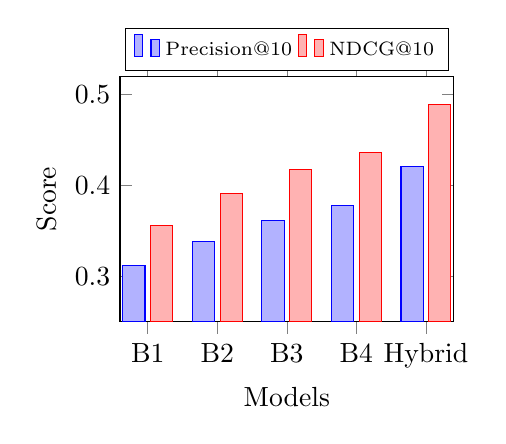
\begin{tikzpicture}
\begin{axis}[
width=0.48\textwidth,
height=4.7cm,
ybar,
bar width=8pt,
ymin=0.25,
ymax=0.52,
legend style={at={(0.5,1.02)},anchor=south,legend columns=2,font=\scriptsize},
symbolic x coords={B1,B2,B3,B4,Hybrid},
xtick=data,
ylabel={Score},
xlabel={Models},
]
\addplot coordinates {(B1,0.312) (B2,0.338) (B3,0.361) (B4,0.378) (Hybrid,0.421)};
\addplot coordinates {(B1,0.356) (B2,0.391) (B3,0.417) (B4,0.436) (Hybrid,0.489)};
\legend{Precision@10,NDCG@10}
\end{axis}
\end{tikzpicture}
\caption{Ranking quality comparison across baselines and hybrid model.}
\label{fig:bar}
\end{figure}

The hybrid model improves Precision@10 by 13.8\% over the best non-hybrid baseline and increases acceptance rate by 15.4\%. Gains are most visible in mid-tier freelancers, indicating reduced popularity bias compared with rule-based ranking.

\subsection{Ablation Study}
Removing collaborative features decreases NDCG@10 by 5.3\%, while removing trust/reliability signals drops acceptance rate by 4.7\%. This confirms that semantic matching alone is insufficient for marketplace outcomes.

\section{Discussion and Conclusion}
This work demonstrates that intelligent freelancer--project matching benefits from hybrid modeling that combines semantic relevance, collaborative behavior, and reliability-aware ranking. Beyond offline metric gains, the system provides operational value by improving project start quality and reducing mismatched proposals.

Future work includes online contextual bandits for exploration-exploitation balance, fairness constraints across emerging freelancers, and graph neural features from project-skill-user interaction networks. Integrating causal uplift estimation may further optimize for long-term marketplace health rather than short-term clicks.

\section*{Acknowledgment}
The authors thank the Department of Computer Applications and project mentors for guidance and infrastructure support.

\begin{thebibliography}{99}
\bibitem{lops2011} P. Lops, M. de Gemmis, and G. Semeraro, ``Content-based Recommender Systems: State of the Art and Trends,'' in \textit{Recommender Systems Handbook}, Springer, 2011.
\bibitem{koren2009} Y. Koren, R. Bell, and C. Volinsky, ``Matrix Factorization Techniques for Recommender Systems,'' \textit{Computer}, vol. 42, no. 8, pp. 30--37, 2009.
\bibitem{rendle2009} S. Rendle, C. Freudenthaler, Z. Gantner, and L. Schmidt-Thieme, ``BPR: Bayesian Personalized Ranking from Implicit Feedback,'' in \textit{UAI}, 2009.
\bibitem{burges2010} C. Burges, ``From RankNet to LambdaRank to LambdaMART: An Overview,'' Microsoft Research Technical Report, 2010.
\bibitem{devlin2019} J. Devlin, M.-W. Chang, K. Lee, and K. Toutanova, ``BERT: Pre-training of Deep Bidirectional Transformers for Language Understanding,'' in \textit{NAACL}, 2019.
\bibitem{guo2017} H. Guo, R. Tang, Y. Ye, Z. Li, and X. He, ``DeepFM: A Factorization-Machine based Neural Network for CTR Prediction,'' in \textit{IJCAI}, 2017.
\bibitem{ekstrand2022} M. D. Ekstrand, A. Das, R. Burke, and F. Diaz, ``Fairness in Recommender Systems,'' in \textit{Recommender Systems Handbook}, Springer, 2022.
\bibitem{chen2016} T. Chen and C. Guestrin, ``XGBoost: A Scalable Tree Boosting System,'' in \textit{KDD}, 2016.
\end{thebibliography}

\end{document}
